\documentclass[a4paper,12pt]{article} 
\usepackage{geometry}
\usepackage{wrapfig}
\geometry{
	a4paper,
	total={170mm,257mm},
	left=10mm,
	right=10mm,
	top=20mm,
}
\usepackage{titlesec}
\titlelabel{\thetitle.\quad} %точка в section

%%% Работа с русским языком
\usepackage{cmap}                           % поиск в PDF
\usepackage{mathtext} 			 	       % русские буквы в формулах
\usepackage[T2A]{fontenc}               % кодировка
\usepackage[utf8]{inputenc}              % кодировка исходного текста
\usepackage[english,russian]{babel}  % локализация и переносы

%Математика
\usepackage{amsmath,amsfonts,amssymb,amsthm,mathtools} % AMS
\usepackage{icomma} % "Умная" запятая

%% Шрифты
\usepackage{euscript}	 % Шрифт Евклид
\usepackage{mathrsfs} % Красивый матшрифт

%% Команды
\DeclareMathOperator{\const}{\mathop{const}}

%% Перенос знаков в формулах
\newcommand*{\hm}[1]{#1\nobreak\discretionary{}
	{\hbox{$\mathsurround=0pt #1$}}{}}

%%% Заголовок
\author{Шерхалов Денис Б02-204}
\title{Лабораторная работа 3.3.1 \\
	\textbf{Измерение удельного заряда электрона методом магнетрона}}
\date{\today}

\begin{document}
	
	{\Large \maketitle}

	\paragraph*{Цель работы:} определение отношения заряда электрона к его массе $e/m$ методом магнетрона. 
	\paragraph*{В работе используются:} электронная лампа с цилиндрическим анодом; универсальный стабилизированный источник постоянного и переменного напряжений; соленоид; миллиамперметр; амперметр и вольтметр постоянного тока.
	
	\section{Введение}
	В методе магнетрона отношение $e / m$ измеряется на основе исследования движения электрона в скрещенных электрическом и магнитном полях, перпендикулярных друг другу. Название метода связано с тем, что такая конфигурация электрического и магнитного полей реализуется в магнетронах --- генераторах электромагнитных колебаний сверхвысоких частот.

	Для уяснения идеи метода магнетрона, рассмотрим вначале движение заряда в <<плоском магнетроне>>б который можно представить себе в виде плоского конденсатора, помещённого в магнитное поле так, что $\boldsymbol{E} \perp \boldsymbol{B}$. При этом отрицательная пластина конденсатора играет роль катода, положительная соответственно анода.  Если бы магнитого поля не было, то все электроны, вылетевшие без начальной из катода такого плоского диода, попадали бы на анод. При наличии магнитного поля траектории электронов искривляются, вследствие чего при достаточно большом магнитном поле ни один электрон не достигнет анода.
	Для заданного напряжения между катодом и анодом существует некоторое критическое значение магнитной индукции $B_\text{кр}$, при котором траектории касаются поверхности анода. Если $B < B_\text{кр}$, то все электроны достигают анода и ток через магнетрон имеет то же значение, что и без магнитного поля. Если же $B > B_\text{кр}$, то электроны не достигают анода и ток через лампу равен нулю.

	Рассчитаем это критическое значение индукции магнитного поля. Уравнения движения электрона в нашем случае имеет вид
	$$m \frac{d v_x}{d t} = e v_y B$$
	$$m \frac{d v_y}{d t} = e E - e v_x B$$
	при начальных условиях $x(0) = y(0) = 0, v_x(0) = v_y (0) = 0$.

	Непосредственной подстановкой несложно убедиться в том, что решением системы дифференциальных уравнений с заданными начальными условиями является уравнение циклоиды (в параметрической форме):
	$$x = v t - R \sin \omega t, \quad y = R(1 - \cos \omega t)$$
	где $v = \frac{E}{B}, R = \frac{v}{\omega} = \frac{E m}{e B^2}$.

	Касание анода происходит при $2R = d$ ($d$ --- расстояние между анодом и катодом). Этому значению соответствует критическое поле
	$$B_\text{кр} = \frac{\sqrt{2V}}{d \sqrt{e / m}}$$
	Из последней формулы находим удельный заряд:
	$$\frac{e}{m} = \frac{2V}{d^2 B_\text{кр}^2}$$
	Эта формула позволяет вычислить $e / m$, если при заданном значении напряжения на аноде $V$ 
	найти такое значение магнитного поля, при превышении которого ток в магнитроне отсутствует.

	В настоящей работе отношение $e / m$ для электрона определяется с помощью метода, получившего 
	название <<метод магнетрона>>. Это название связано с тем, что применяемая в работе конфигурация
	электрического и магнитного полей напоминает конфигурацию полей в магнетронах --- генераторах 
	электромагнитных колебаний сверхвысоких частот.

	\begin{figure}[h!]
		\centering{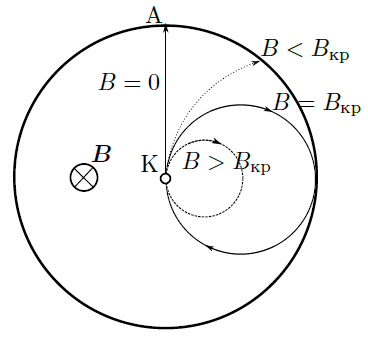
\includegraphics[width=0.5\textwidth]{ris4.png}}
		\caption[]{\label{fig:1} Траектории электронов, вылетающих из катода, при разных значениях индукции магнитного поля}
	\end{figure}	

	Движение электронов в этом случае происходит в кольцевом пространстве, заключённом между катодом и анодом двухэлектродной электронной лампы. Нить накала лампы (катод) располагается вдоль оси цилиндрического анода, так что электрическое поле между катодом и анодом имеет радиальное направление. Лампа помещается внутри соленоида, создающего магнитное поле, параллельное оси лампы.

	Рассмотрим траектории электронов, вылетевших из катода, более подробно. Пусть потенциал анода равен $V_a$. В отсутствие магнитного поля электрон движется прямолинейно по радиусу. При слабом поле траектории несколько искривляются, но электроны всё же попадают на анод. При некотором критическом значении индукции магнитного поля $B_\text{кр}$ траектории искривляются настолькко, что касаются анода. Наконец, при $B > B_\text{кр}$ электроны вовсе не попадают на анод и возвращаются к катоду. Величину $B_\text{кр}$ нетрудно найти по формуле, приведённой выше, заметив, что в этом случае радиальная скорость электрона $\dot r$ при $r = r_a$ (при радиусе анода) обращается в нуль:
	$$V_a = \frac{e B_\text{кр}^2 r_a^2}{8 m}$$
	Преобразуя это выражение, найдём 
	$$\frac{e}{m} = \frac{8 V_a}{B_\text{кр}^2 r_a^2}$$
	
	Эта формула позволяет вычислять $e / m$, если при заданном $V_a$ найдено значение магнитного поля (или, наоборот, при заданном $B$ такое значение $V_a$), при котором электроны перестают попадать на анод.
	\begin{figure}[h!]
		\centering{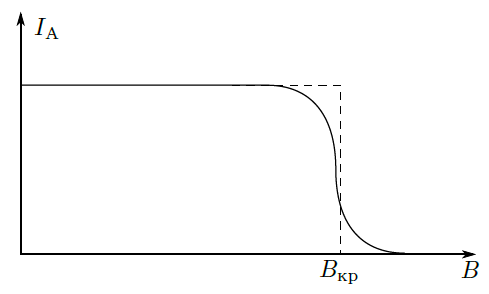
\includegraphics[width=0.5\textwidth]{ris5.png}}
		\caption[]{\label{fig:2} Зависимость анодного тока от индукции магнитного поля в соленоиде}
	\end{figure}	
	
	До сих пор мы рассматривали идеальный случай, когда при $B < B_\text{кр}$ все электроны без исключения попадают на анод, а при $B > B_\text{кр}$ все они возвращаются на катод, не достигнув анода. Анодный ток $I_a$ c увеличением магнитного поля изменялся бы при этом так, как это изображено на риснуке выше пунктирной линией. В реальных условиях невозможно обеспечить полную коаксиальность анода и катода, вектор индукции магнитного поля всегда несколько наклонён по отношению к катоду, магнитное поле не вполне однородно и так далее. Все эти причины приводят к сглаживанию кривой на рисунке выше и она приобретает вид сплошной линии. В хорошо собранной установке перелом функции $I_a = f(B)$ остаётся, однако, достаточно резким и с успехом может быть использован для измерения $e / m$.

	Итого, удельный заряд электрона определяется по формуле
	\begin{equation}
		\dfrac{e}{m_e} = \dfrac{8V_a}{B_{\text{кр}}^2r_a^2},
	\end{equation}
	где $V_a$ - анодное напряжение, $B_{\text{кр}}$ - критическое поле, $r_a$ - радиус анода.
	\subsection*{Экспериментальная установка}
	
	Два крайних цилиндра изолированы от среднего небольшими зазорами и используются для устранения краевых эффектов на торцах среднего цилиндра, ток с которого используется при измерениях. В качестве катода используется тонкая вольфрамовая проволока. Катод разогревается переменным током, отбираемым от стабилизированного источника питания. 
	
	С этого же источника на анод лампы подается напряжение, регулируемое с помощью потенциометра и измеряемое вольтметром.
	
	Индукция магнитного поля в соленоиде рассчитывается по току $I_m$, протекающему через обмотку соленоида. Коэффициент пропорциональности между ними указан в установке.
	
	Лампа закреплена в соленоиде. Магнитное поле в соленоиде создается постоянным током, сила которого регулируется ручками источника питания и измеряется амперметром.

	\begin{figure}[h!]
		\centering{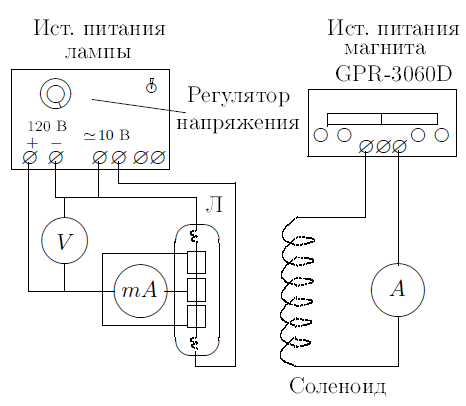
\includegraphics[width=0.5\textwidth]{6.png}}
		\caption[]{\label{fig:3} Схема установки для измерений $e/m$ методом магнетрона}
	\end{figure}	

	\section{Выполнение}
	
	\begin{enumerate}

		\item Запишем параметры установки:
		$$K = 3,5 \cdot 10^{-2} \; Тл/А \qquad r_a = 12\;мм \qquad \Delta I_a = 1\;дел = 4\;мкА \qquad \Delta I_m = 1\;дел = 4\;мА$$
		В таком случае, $\Delta B = K \cdot \Delta I_m = 0.14\;мТл \sim 0.1\;мТл$

		\item Установим на аноде лампы потенциал $V_a = 70 \, В$. Снимем зависимость анодного тока $I_a$ от тока $I_m$, 
		протекающего через соленоид, при различных напряжениях на аноде лампы, построим графики (см. в приложении) для каждого 
		напряжения на аноде и по результатам измерений рассчитаем удельный заряд электрона:
		\begin{table}[h!]
			\caption{$V_a = 70 \, В$}
			\begin{center}
				\begin{tabular}{|*{18}{l|}} \hline
					$I_a$, дел & 75 & 75 & 75 &	74 & 73 & 62 & 11 & 5 & 3 & 1 & 1 & 1 & 1 & 0 & 0 & 0 & 0 \\ \hline
					$I_a$, мкА & 300 & 300 & 300 & 296 & 292 & 248 & 44 & 20 & 12 & 4 & 4 & 4 & 4 & 0 & 0 & 0 & 0 \\ \hline
					$I_m$, дел & 8 & 20 & 29 &	30 & 31 & 32 & 33 & 34 & 35 & 36 & 37 & 38 & 39 & 40 & 41 & 42 & 45 \\ \hline
					$I_m$, мА & 32 & 80 & 116 & 120 & 124 & 128 & 132 & 136 & 140 & 144 & 148 & 152 & 156 & 160 & 164 & 168 & 180 \\ \hline
					$B$, мТл& 1.1 & 2.8 & 4.1 & 4.2 & 4.3 & 4.5 & 4.6 & 4.8 & 4.9 & 5.0 & 5.2 & 5.3 & 5.5 & 5.6 & 5.7 & 5.9 & 6.3 \\ \hline	
				\end{tabular}	
			\end{center}
		\end{table}

		\begin{table}[h!]
			\caption{$V_a = 80 \, В$}
			\begin{center}
				\begin{tabular}{|*{18}{l|}} \hline
					$I_a$, дел & 77 & 76 & 76 &	76 & 76 & 76 & 65 & 17 & 8 & 4 & 2 & 1 & 1 & 1 & 1 & 1 & 0 \\ \hline
					$I_a$, мкА & 308 & 304 & 304 & 304 & 304 & 304 & 260 & 68 & 32 & 16 & 8 & 4 & 4 & 4 & 4 & 4 & 0 \\ \hline
					$I_m$, дел & 15 & 20 & 24 &	27 & 30 & 33 & 34 & 35 & 36 & 37 & 38 & 39 & 40 & 42 & 43 & 45 & 46 \\ \hline
					$I_m$, мА & 60 & 80 & 96 & 108 & 120 & 132 & 136 & 140 & 144 & 148 & 152 & 156 & 160 & 168 & 172 & 180 & 184 \\ \hline
					$B$, мТл & 2.1 & 2.8 & 3.4 & 3.8 & 4.2 & 4.6 & 4.8 & 4.9 & 5.0 & 5.2 & 5.3 & 5.5 & 5.6 & 5.9 & 6.0 & 6.3 & 6.4 \\ \hline
				\end{tabular}	
			\end{center}
		\end{table}
		
		\begin{table}[h!]
			\caption{$V_a = 90 \, В$}
			\begin{center}
				\begin{tabular}{|*{16}{l|}} \hline
					$I_a$, дел & 75 & 75 & 75 &	75 & 71 & 26 & 10 & 6 & 3 & 2 & 1 & 1 & 1 & 1 & 0 \\ \hline
					$I_a$, мкА & 300 & 300 & 300 & 300 & 284 & 104 & 40 & 24 & 12 & 8 & 4 & 4 & 4 & 4 & 0 \\ \hline
					$I_m$, дел & 26 & 30 & 33 &	34 & 35 & 36 & 37 & 38 & 39 & 40 & 41 & 42 & 43 & 44 & 45 \\ \hline
					$I_m$, мА & 104 & 120 & 132 & 136 & 140 & 144 & 148 & 152 & 156 & 160 & 164 & 168 & 172 & 176 & 180 \\ \hline
					$B$, мТл & 3.6 & 4.2 & 4.6 & 4.8 & 4.9 & 5.0 & 5.2 & 5.3 & 5.5 & 5.6 & 5.7 & 5.9 & 6.0 & 6.2 & 6.3 \\ \hline
				\end{tabular}	
			\end{center}
		\end{table}
		
		\begin{table}[h!]
			\caption{$V_a = 100 \, В$}
			\begin{center}
				\begin{tabular}{|*{18}{l|}} \hline
					$I_a$, дел & 76 & 76 & 76 &	76 & 66 & 30 & 12 & 6 & 3 & 2 & 2 & 2 & 1 & 1 & 1 & 0 & 0 \\ \hline
					$I_a$, мкА & 304 & 304 & 304 & 304 & 264 & 120 & 48 & 24 & 12 & 8 & 8 & 8 & 4 & 4 & 4 & 0 & 0 \\ \hline
					$I_m$, дел & 33 & 34 & 35 &	36 & 37 & 38 & 39 & 40 & 41 & 42 & 43 & 44 & 45 & 46 & 47 & 48 & 49 \\ \hline
					$I_m$, мА & 132 & 136 & 140 & 144 & 148 & 152 & 156 & 160 & 164 & 168 & 172 & 176 & 180 & 184 & 188 & 192 & 196 \\ \hline
					$B$, мТл & 4.6 & 4.8 & 4.9 & 5.0 & 5.2 & 5.3 & 5.5 & 5.6 & 5.7 & 5.9 & 6.0 & 6.2 & 6.3 & 6.4 & 6.6 & 6.7 & 6.9\\ \hline
				\end{tabular}	
			\end{center}
		\end{table}

		\begin{table}[h!]
			\caption{$V_a = 100 \, В$}
			\begin{center}
				\begin{tabular}{|*{18}{l|}} \hline
					$I_a$, дел & 78 & 77 & 76 & 76 & 75 & 30 &	16 & 8 & 4 & 3 & 2 & 2 & 2 & 1 & 1 & 0 & 0 \\ \hline
					$I_a$, мкА & 312 & 308 & 304 & 304 & 300 & 120 & 64 & 32 & 16 & 12 & 8 & 8 & 8 & 4 & 4 & 0 & 0 \\ \hline
					$I_m$, дел & 35 & 36 & 37 &	38 & 39 & 40 & 41 & 42 & 43 & 44 & 45 & 46 & 47 & 48 & 49 & 50 & 51 \\ \hline
					$I_m$, мА & 140 & 144 & 148 & 152 & 156 & 160 & 164 & 168 & 172 & 176 & 180 & 184 & 188 & 192 & 196 & 200 & 204 \\ \hline
					$B$, мТл & 4.9 & 5.0 & 5.2 & 5.3 & 5.5 & 5.6 & 5.7 & 5.9 & 6.0 & 6.2 & 6.3 & 6.4 & 6.6 & 6.7 & 6.9 & 7.0 & 7.1 \\ \hline
				\end{tabular}	
			\end{center}
		\end{table}

		\newpage

		\item Построим график зависимости $B_{кр}^2$ от $V$ и по углу коэффициента наклона графика определим удельный заряд электрона:
		
		\begin{table}[h!]
			\caption{Значения $B_{кр}$ и $V$. $\Delta V =  2\;В$, $\Delta B_{кр} =  0.1\;мТл$}
			\begin{center}
				\begin{tabular}{|*{6}{l|}} \hline
					$V$, В & 70 & 80 & 90 & 100 & 110 \\ \hline
					$B_{кр}$, мТл & 4.5 & 4.8 & 5.0 & 5.3 & 5.6 \\ \hline 
				\end{tabular}	
			\end{center}
		\end{table}

		\begin{figure}[h!]
			\centering{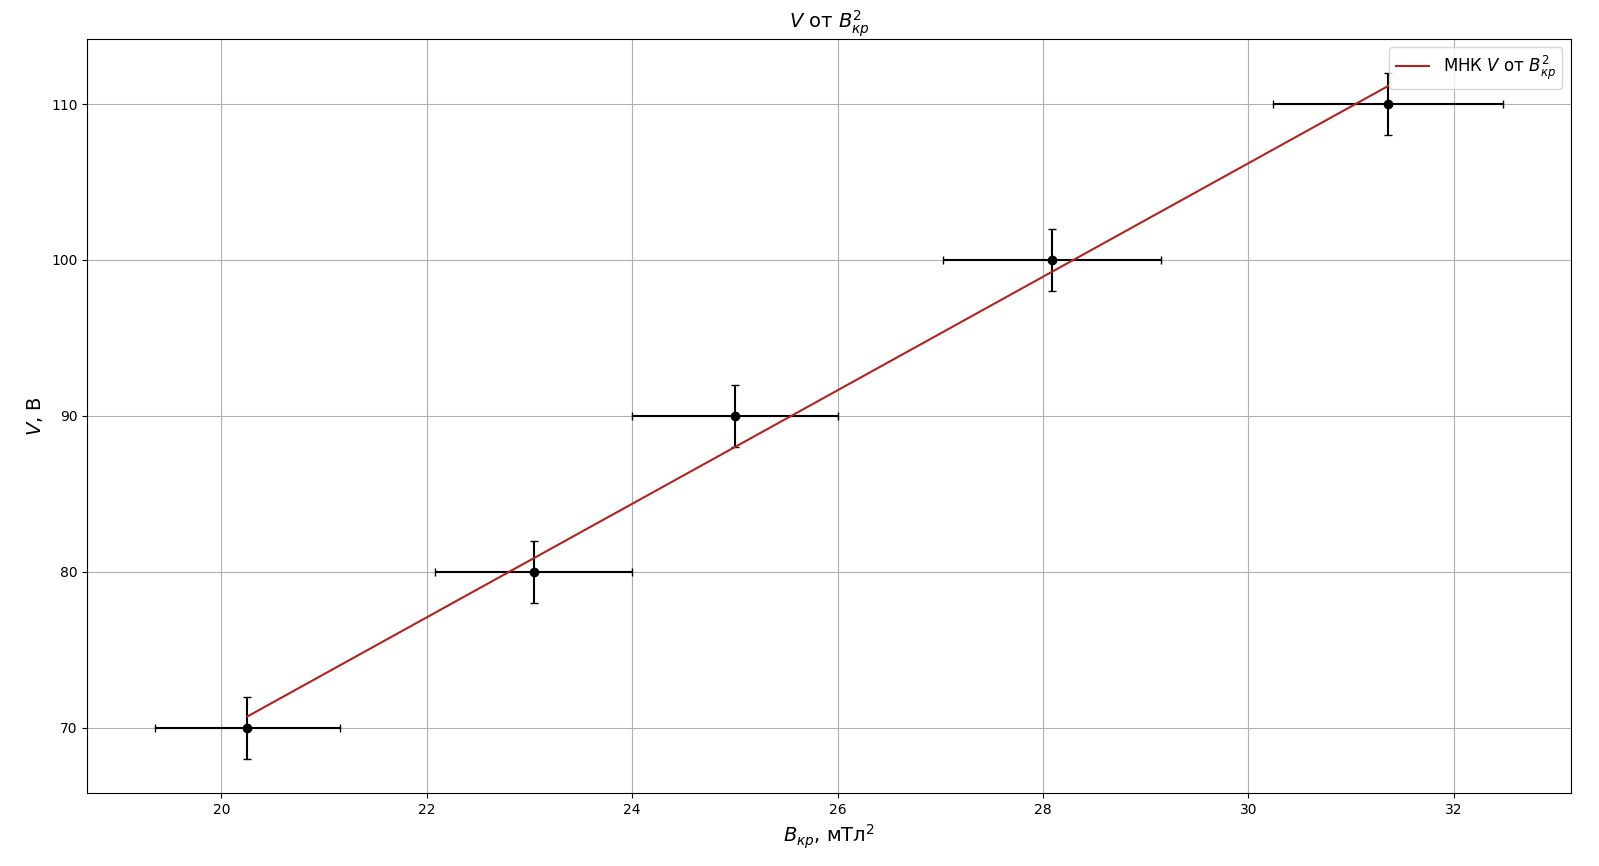
\includegraphics[width=1\textwidth]{gr.png}}
		\end{figure}
		
		Угловой коэффициент графика $k = 3.6 \pm 0.5 \; \dfrac{В}{мТл^2}$ . Отсюда находим:
	$$\frac{e}{m} = (2.0 \pm 0.3) \cdot 10^{11} \frac{\text{Кл}}{\text{кг}}$$
		

\end{enumerate}

\section{Вывод}
Полученный экспериментальным путём относительный заряд электрона 
$e / m = (2.0 \pm 0.3) \cdot 10^{11} \frac{\text{Кл}}{\text{кг}}$ с некоторой точностью совпадает с табличным $e / m =  1.7 \cdot 10^{11} \frac{\text{Кл}}{\text{кг}}$, что показывает правильность наших теоретических выкладок.

\newpage 

\begin{figure}[h!]
	\centering{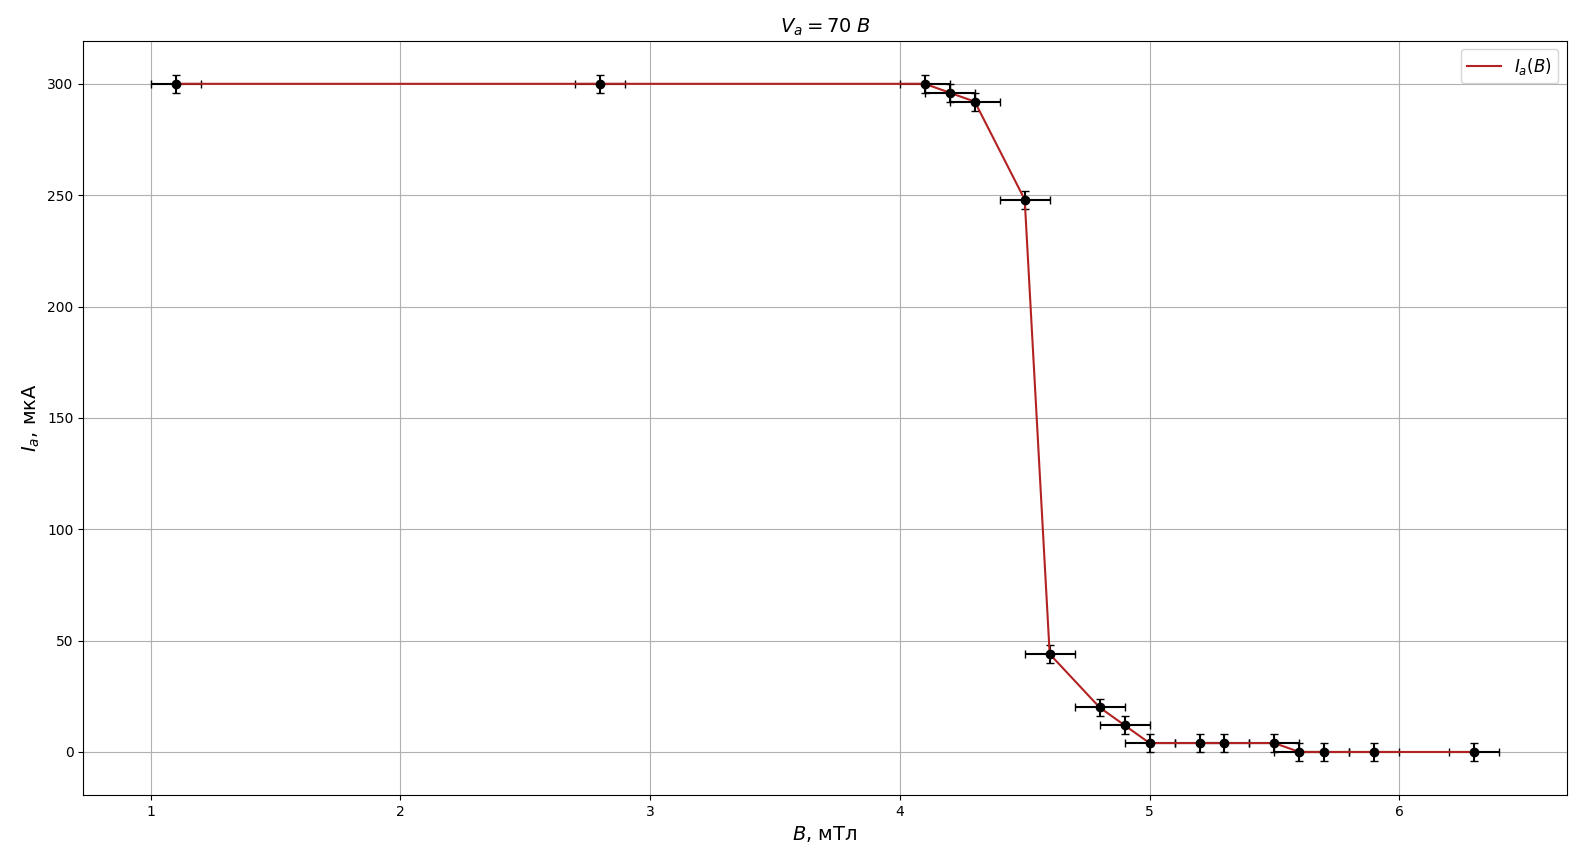
\includegraphics[width=1\textwidth]{gr1.png}}
\end{figure}
\begin{figure}[h!]
	\centering{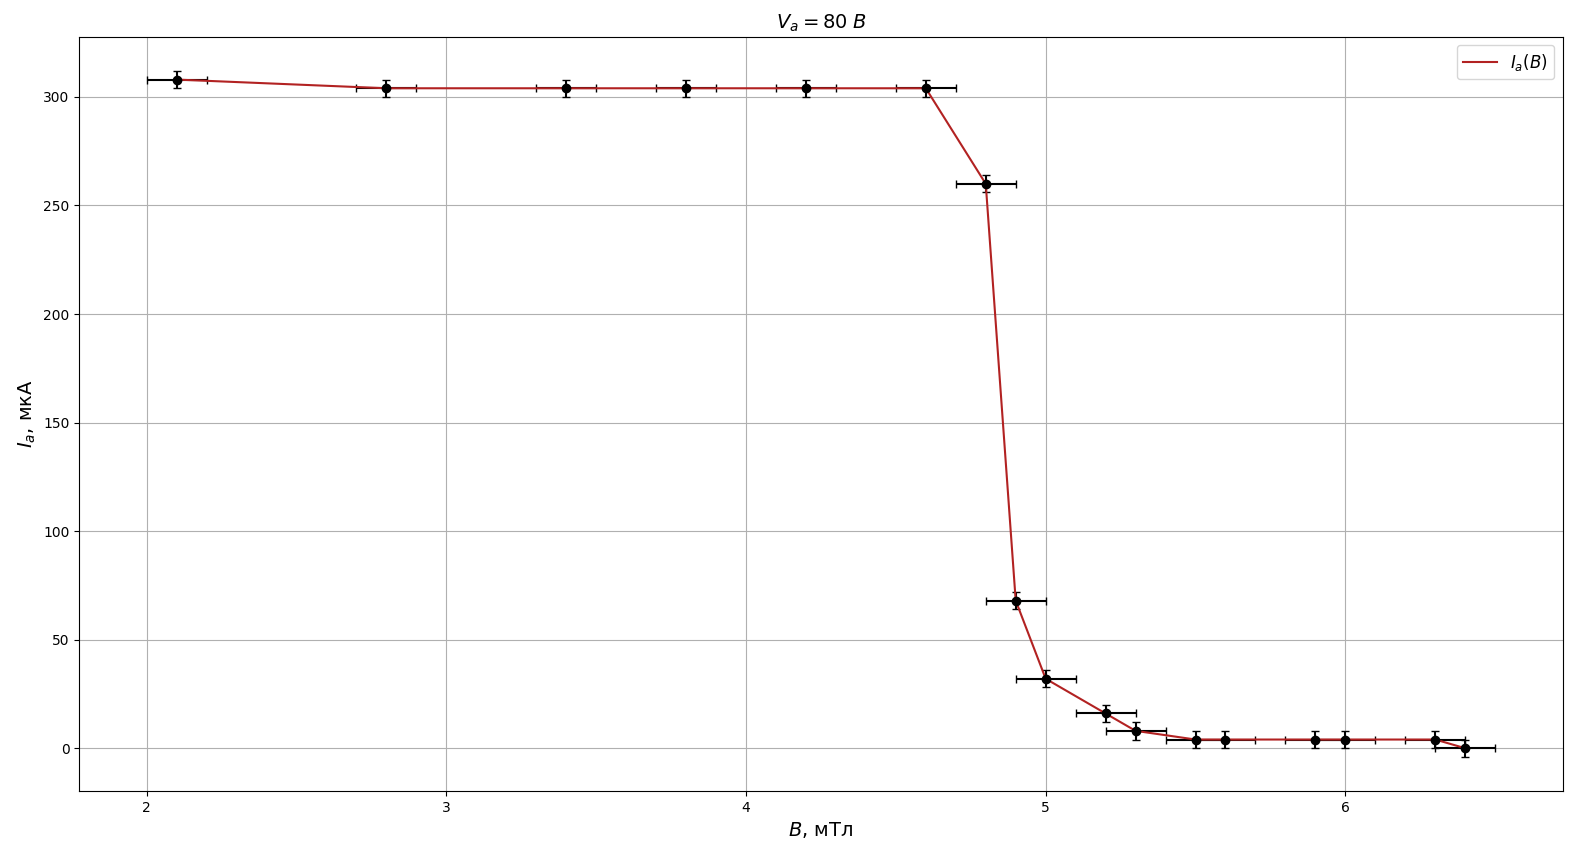
\includegraphics[width=1\textwidth]{gr2.png}}
\end{figure}
\begin{figure}[h!]
	\centering{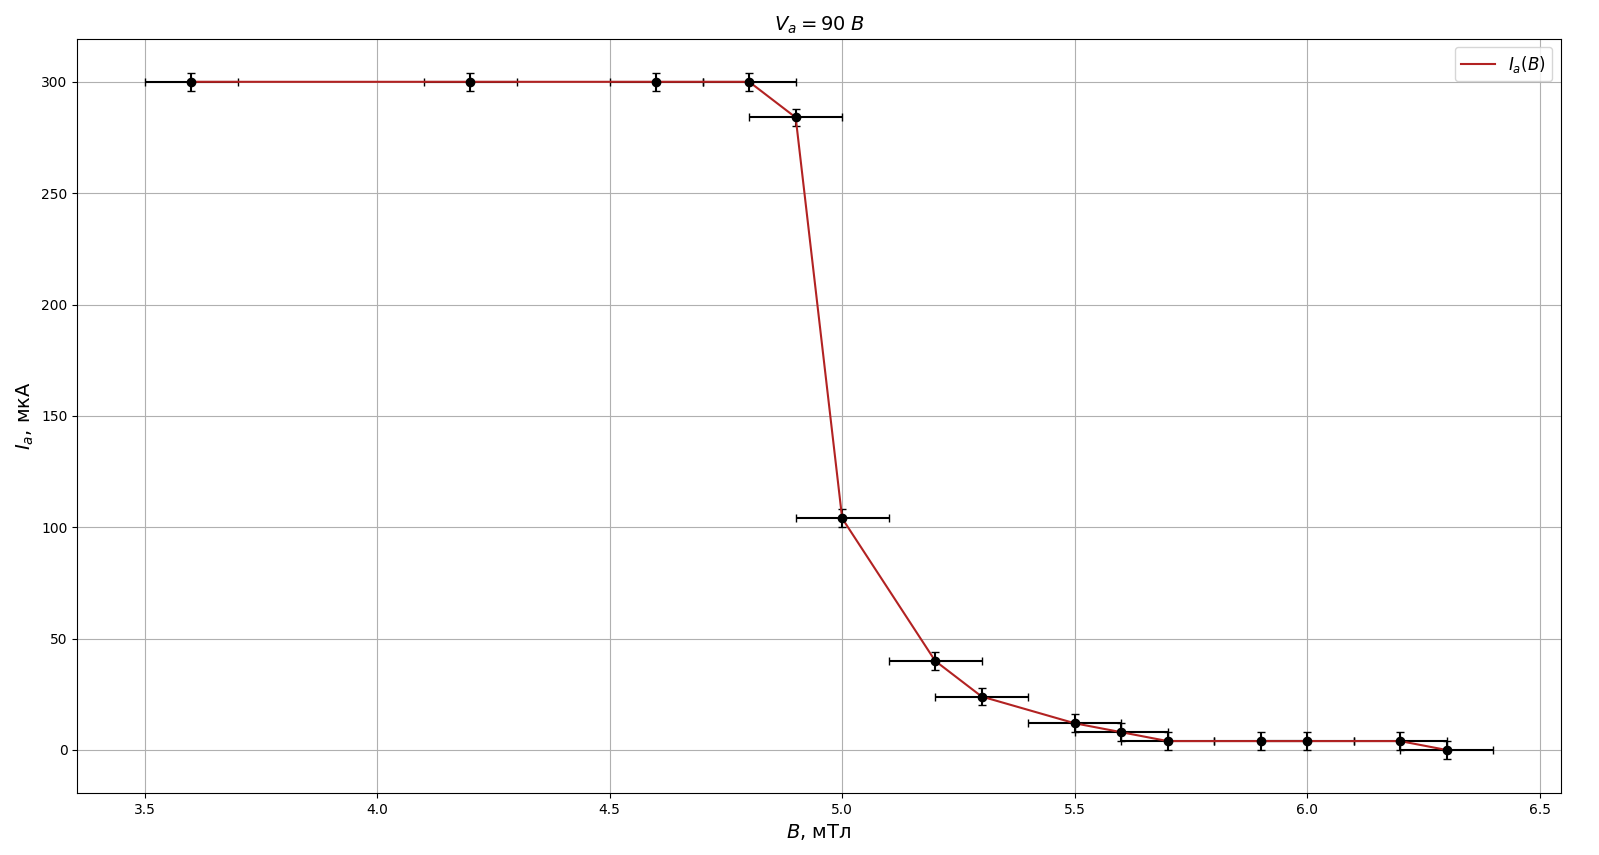
\includegraphics[width=1\textwidth]{gr3.png}}
\end{figure}
\begin{figure}[h!]
	\centering{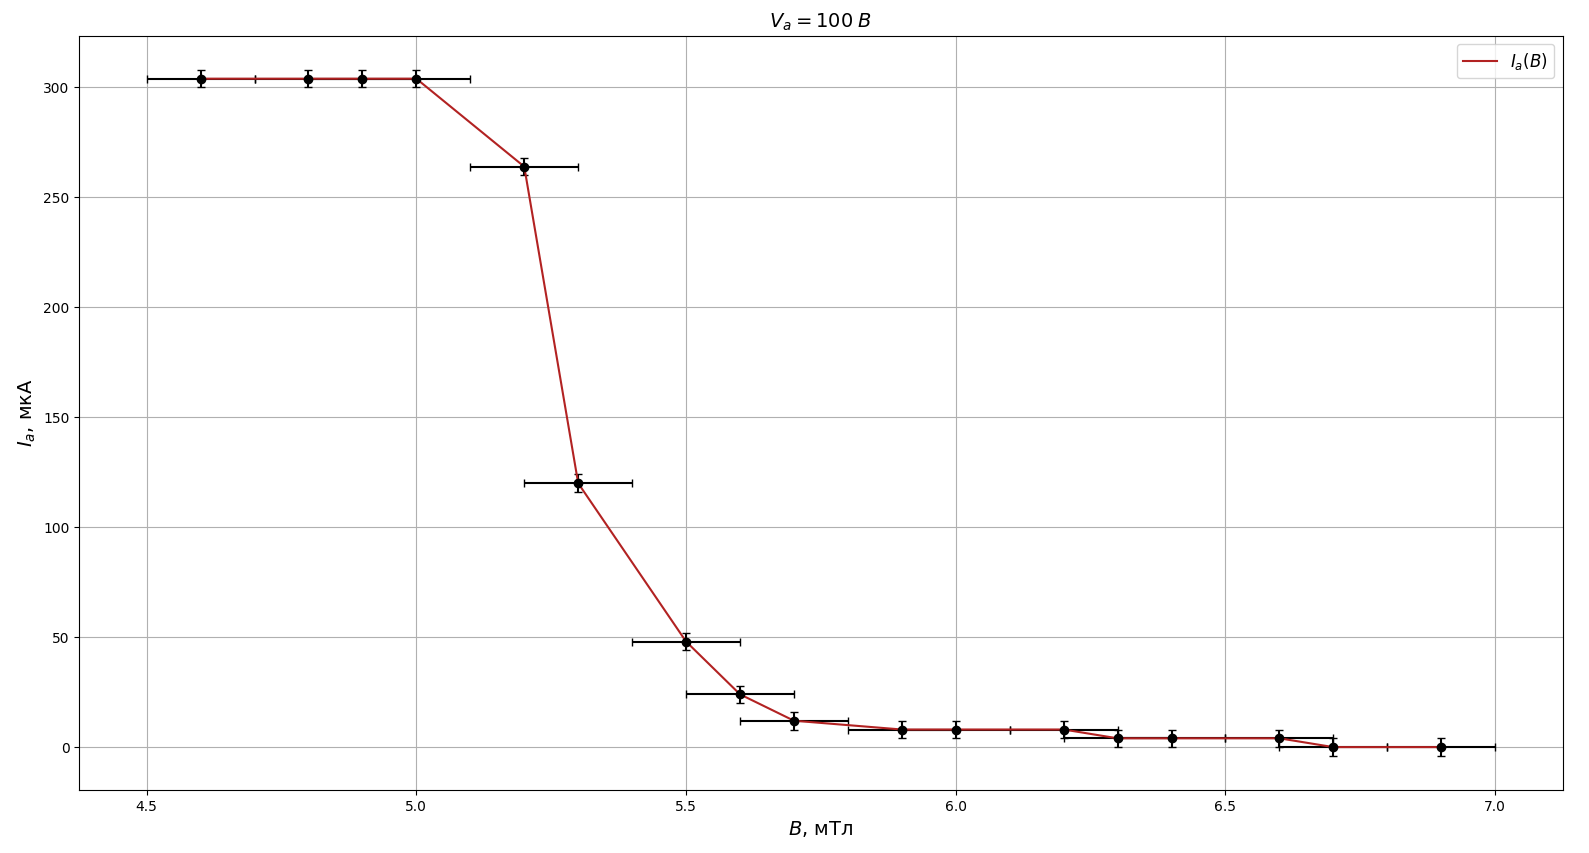
\includegraphics[width=1\textwidth]{gr4.png}}
\end{figure}
\begin{figure}[h!]
	\centering{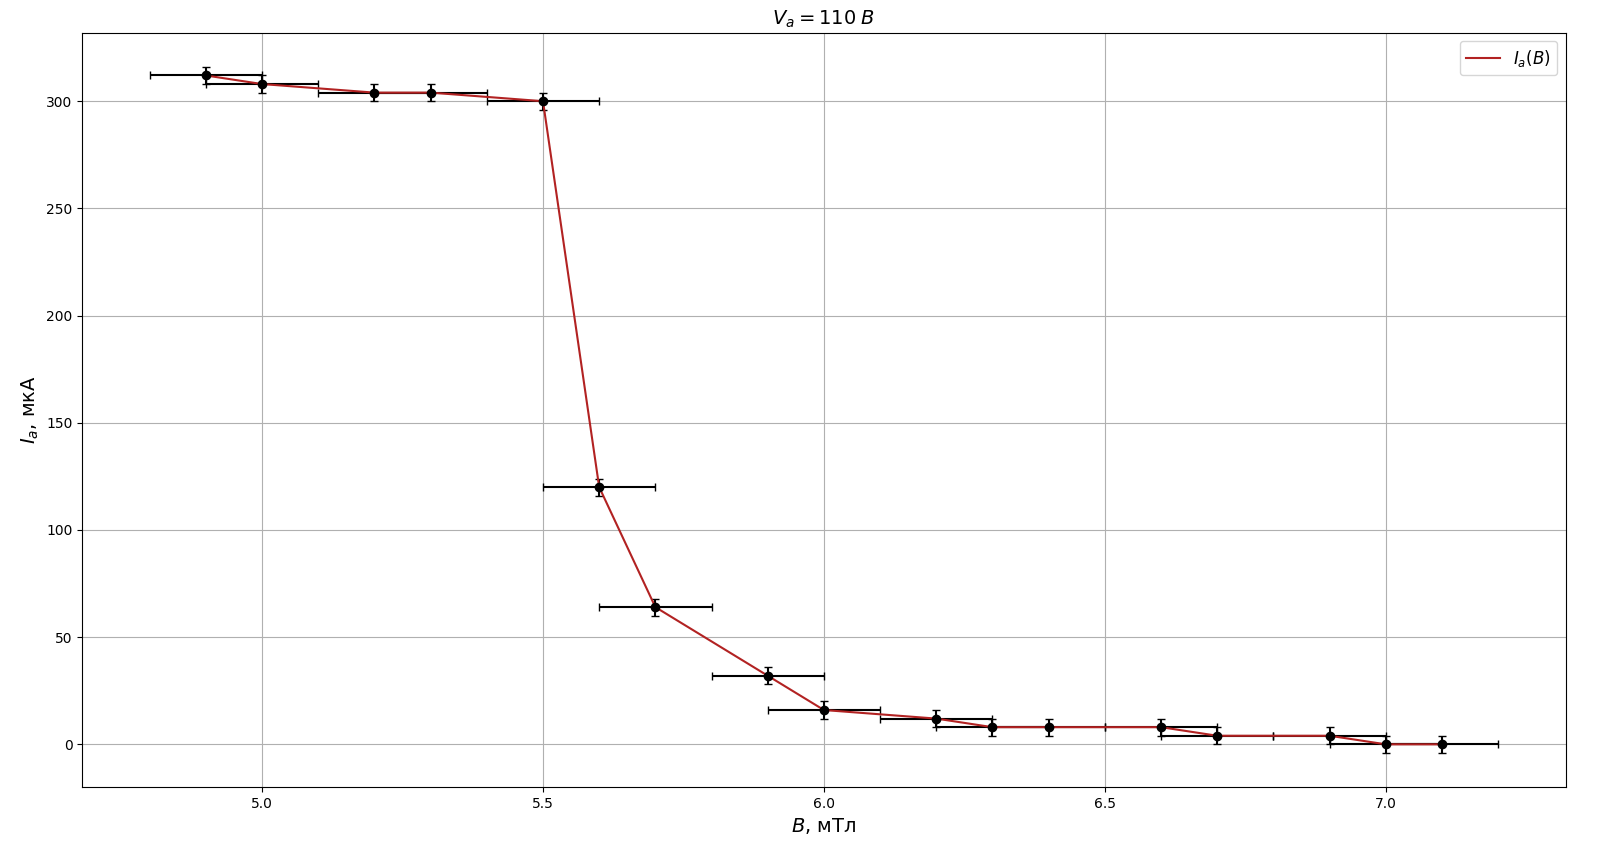
\includegraphics[width=1\textwidth]{gr5.png}}
\end{figure}

\end{document}